% !TeX program = lualatex
% ================================================================
% Polish Parallel Text Version of AppliedRatioCrossTopics
%
% Generated by the server using the following settings:
%
%   language            Polish (pol)
%   text direction      left to right
%   font                Noto Serif
%   fallback font       Noto Serif
%   built from          latex/worksheets/ratioAndProportion/crossTopic/appliedRatioCrossTopics.tex
%   vocabulary key      latex/worksheets/ratioAndProportion/crossTopic/appliedRatioCrossTopics/L2/pol/appliedRatioCrossTopics_polishKey.tex
%   tier 3 vocabulary   green   RGB 0 128 0
%   English text        black   RGB 0 0 0
%   Polish text         purple  RGB 112 48 160
%   layout macros       version 3
%
% Please don't edit any information in this comment block - the server
% compares it against the current settings and rebuilds this file when
% they differ, so changes here would be overwritten. However, feel free
% to make updates to the LaTeX below if you want to edit it.
% ================================================================

\documentclass[12pt]{article}
% ================================================================
% Copied from the English sheet this was translated from, so that
% anything it sets up for itself still works here
% ================================================================
\usepackage{amsmath}
\usepackage{tikz}
\usepackage{enumitem}
\usepackage[margin=1in]{geometry}

\title{Applied Ratio Extension Problems}
\date{}

% Characters this language's font has not got are borrowed from another,
% rather than being silently dropped - see docs/translated-sheet-latex.md
\directlua{%
  if luaotfload and luaotfload.add_fallback then
    luaotfload.add_fallback("eallatinfallback",
      { "Noto Serif:mode=harf;" })
  else
    tex.error("this luaotfload is too old to register a fallback font")
  end
}
\usepackage[english]{babel}
\babelprovide[import]{polish}
\babelfont[polish]{rm}[Renderer=Harfbuzz, BoldFont={Noto Serif}, ItalicFont={Noto Serif}, BoldItalicFont={Noto Serif}, RawFeature={fallback=eallatinfallback}]{Noto Serif}
\babelfont[polish]{sf}[Renderer=Harfbuzz, BoldFont={Noto Serif}, ItalicFont={Noto Serif}, BoldItalicFont={Noto Serif}, RawFeature={fallback=eallatinfallback}]{Noto Serif}
\newcommand{\ealtext}[1]{\foreignlanguage{polish}{#1}}
\newcommand{\ealtextblock}[1]{{\raggedright\foreignlanguage{polish}{#1}\par}}
% ================================================================
% EAL layout helpers
% ================================================================
\usepackage{xcolor}

\definecolor{ealkeycolour}{RGB}{0,128,0}
\definecolor{ealenglish}{RGB}{0,0,0}
\definecolor{ealtwocolour}{RGB}{112,48,160}

\newsavebox{\ealboxen}
\newsavebox{\ealboxtr}
\newlength{\ealglosswd}
\newlength{\ealglossraise}
\setlength{\ealglossraise}{1.15em}

% a tier 3 word, in English and in translation alike
\newcommand{\ealkey}[1]{\textcolor{ealkeycolour}{#1}}
\newcommand{\ealkeytr}[1]{\textcolor{ealkeycolour}{\ealtext{#1}}}

% One translated word above one English word. Built from kernel
% primitives, never a tabular, which would break wherever the sheet
% loads array, booktabs or tabularx. The box is as wide as the wider of
% the two, so a long translation pushes its neighbours aside instead of
% overlapping them, and it claims its full height so a table row or a
% TikZ node makes room for it.
\newcommand{\ealgloss}[2]{%
  \sbox{\ealboxen}{\ealkey{#1}}%
  \sbox{\ealboxtr}{\small\textcolor{ealtwocolour}{\ealtext{#2}}}%
  \setlength{\ealglosswd}{\wd\ealboxen}%
  \ifdim\wd\ealboxtr>\ealglosswd\setlength{\ealglosswd}{\wd\ealboxtr}\fi
  \leavevmode
  \makebox[\ealglosswd][c]{%
    \makebox[0pt][c]{\usebox{\ealboxen}}%
    \makebox[0pt][c]{\raisebox{\ealglossraise}{\usebox{\ealboxtr}}}%
  }%
}

% opens up line spacing around a block of glosses, so the raised
% translations sit clear of the line above
\newenvironment{ealglossed}{\par\linespread{2.1}\selectfont\ignorespaces}{\par}

% a whole translated sentence above its English counterpart. block level,
% so it does not belong inside a tabular cell
\newcommand{\ealpara}[2]{%
  \par\addvspace{0.5\baselineskip}%
  {\color{ealtwocolour}\ealtextblock{#1}}%
  \penalty200
  {\color{ealenglish}#2\par}%
  \addvspace{0.5\baselineskip}%
}

\begin{document}

\maketitle

\ealpara{Pytania o przepisy -- przeszłość}{Recipe Questions Past}
\section*{Recipe Questions Past}

\begin{enumerate}
\item \ealpara{Przepis na muffiny robi 12 mufin z następujących składników:}{A muffin recipe makes 12 muffins with the following ingredients:}
    \begin{itemize}
    \item \ealpara{300 g mąki}{300g flour}
    \item \ealpara{200 g cukru}{200g sugar}
    \item \ealpara{2 jajka (około 100 g)}{2 eggs (approx. 100g)}
    \item \ealpara{250 ml mleka}{250ml milk}
    \end{itemize}
    \ealpara{Chcesz zwiększyć wydajność o 50\%. Oblicz nowe ilości wszystkich składników.}{You want to increase the yield by 50\%. Calculate the new quantities for all ingredients.}

\item \ealpara{Przepis na sos jest dla 4 osób:}{A sauce recipe serves 4 people:}
    \begin{itemize}
    \item \ealpara{400 ml passaty pomidorowej}{400ml tomato passata}
    \item \ealpara{2 ząbki czosnku (20 g)}{2 cloves garlic (20g)}
    \item \ealpara{100 ml oliwy z oliwek}{100ml olive oil}
    \item \ealpara{50 g świeżej bazylii}{50g fresh basil}
    \end{itemize}
    \ealpara{Chcesz zrobić tylko 75\% oryginalnego przepisu. Oblicz nowe ilości.}{You only want to make 75\% of the original recipe. Calculate the new quantities.}

\item \ealpara{Przepis na ciasto dla 6 osób wymaga:}{A cake recipe that serves 6 people requires:}
    \begin{itemize}
    \item \ealpara{240 g mąki}{240g flour}
    \item \ealpara{180 g masła}{180g butter}
    \item \ealpara{150 g cukru}{150g sugar}
    \item \ealpara{3 jajka (150 g)}{3 eggs (150g)}
    \end{itemize}
    \ealpara{Musisz obsłużyć 10 osób. O ile \ealkeytr{procent} musisz zwiększyć przepis? Oblicz wszystkie nowe ilości składników.}{You need to serve 10 people. By what \ealkey{percentage} must you increase the recipe? Calculate all new ingredient quantities.}

\item \ealpara{Po gotowaniu masz 560 g makaronu z przepisu, który został zwiększony o 40\% w stosunku do swojej pierwotnej wielkości. Jaka była pierwotna \ealkeytr{masa} makaronu, który dawał przepis?}{After cooking, you have 560g of pasta from a recipe that was increased by 40\% from its original size. What was the original \ealkey{mass} of pasta the recipe made?}

\newpage{}

\item \ealpara{Przepis na chleb używa:}{A bread recipe uses:}
    \begin{itemize}
    \item \ealpara{1000 g mąki}{1000g flour}
    \item \ealpara{600 ml wody}{600ml water}
    \item \ealpara{20 g soli}{20g salt}
    \item \ealpara{15 g drożdży}{15g yeast}
    \end{itemize}
    \ealpara{Piekarz robi nową partię, używając 850 g mąki po zmniejszeniu przepisu.}{The baker makes a new batch using 850g of flour after reducing the recipe.}
    \begin{enumerate}
    \item \ealpara{O ile \ealkeytr{procent} zmniejszono przepis?}{By what \ealkey{percentage} was the recipe reduced?}
    \item \ealpara{Oblicz nowe ilości wszystkich pozostałych składników.}{Calculate the new quantities for all other ingredients.}
    \end{enumerate}
\end{enumerate}


\ealpara{Pytania o przepisy -- przyszłość}{Recipe Questions Future}
\section*{Recipe Questions Future}

\begin{enumerate}[resume]
\item \ealpara{Robisz kwadratowe brownie. Przepis na blachę 20cm × 20cm używa:}{You are making a square brownie. The recipe for a 20cm × 20cm tray uses:}
    \begin{itemize}
    \item \ealpara{200 g czekolady}{200g chocolate}
    \item \ealpara{150 g masła}{150g butter}
    \item \ealpara{3 jajka}{3 eggs}
    \end{itemize}
    \ealpara{Używasz większej blachy 25cm × 25cm. Oblicz nowe ilości wszystkich składników.}{You are using a larger 25cm × 25cm tray. Calculate the new quantities for all ingredients.}

\item \ealpara{Pieczesz okrągłe ciasto. Oryginalny przepis jest na formę do ciasta o \ealkeytr{średnicy} 20cm i używa:}{You are baking a circular cake. The original recipe is for a cake tin with a \ealkey{diameter} of 20cm and uses:}
    \begin{itemize}
    \item \ealpara{250 g mąki}{250g flour}
    \item \ealpara{200 g cukru}{200g sugar}
    \item \ealpara{4 jajka}{4 eggs}
    \end{itemize}
    \ealpara{Używasz formy o \ealkeytr{średnicy} 30cm. Oblicz nowe ilości.}{You are using a tin with a \ealkey{diameter} of 30cm. Calculate the new quantities.}

\item \ealpara{Robisz dwie prostokątne pizze. Duża pizza ma \ealkeytr{wymiary} 35cm × 25cm. Mała pizza ma \ealkeytr{wymiary} 20cm × 15cm. Przepis na małą pizzę używa:}{You are making two rectangular pizzas. The large pizza has \ealkey{dimensions} 35cm × 25cm. The small pizza has \ealkey{dimensions} 20cm × 15cm. The small pizza recipe uses:}
    \begin{itemize}
    \item \ealpara{200 g sera}{200g cheese}
    \item \ealpara{150 g mąki}{150g flour}
    \item \ealpara{100 ml sosu pomidorowego}{100ml tomato sauce}
    \end{itemize}
    \begin{enumerate}
    \item \ealpara{Jakie jest \ealkeytr{pole} każdej pizzy?}{What is the \ealkey{area} of each pizza?}
    \item \ealpara{Ile każdego składnika potrzebuje duża pizza?}{How much of each ingredient does the large pizza need?}
    \end{enumerate}

\newpage{}

\item \ealpara{Dekorujesz \ealkeytr{obwód} prostokątnego ciasta posypką. Ciasto ma 28cm długości i 18cm szerokości. Jeden gram posypki pokrywa 4cm \ealkeytr{obwodu}.}{You are decorating the \ealkey{perimeter} of a rectangular cake with sprinkles. The cake is 28cm long and 18cm wide. One gram of sprinkles covers 4cm of \ealkey{perimeter}.}
    \begin{itemize}
    \item \ealpara{300 g spodu ciasta}{300g cake base}
    \item \ealpara{200 g lukru}{200g icing}
    \item \ealpara{50 g posypki (pierwotna ilość)}{50g sprinkles (original amount)}
    \end{itemize}
    \begin{enumerate}
    \item \ealpara{Jaki jest \ealkeytr{obwód} twojego ciasta?}{What is the \ealkey{perimeter} of your cake?}
    \item \ealpara{Ile gramów posypki potrzebujesz?}{How many grams of sprinkles do you need?}
    \item \ealpara{Jeśli zrobisz ciasto o podwojonym \ealkeytr{obwodzie}, przez jaki \ealkeytr{dzielnik} powinieneś pomnożyć wszystkie składniki?}{If you make a cake with double the \ealkey{perimeter}, by what \ealkey{factor} should you multiply all ingredients?}
    \end{enumerate}

\item \ealpara{Fantazyjny trójkątny deser ma długości boków 12cm, 12cm i 8cm. Tworzysz \ealkeytr{podobny} deser, w którym wszystkie długości boków są zwiększone o \ealkeytr{współczynnik skali} 1.5.}{A fancy triangular dessert has side lengths 12cm, 12cm, and 8cm. You create a \ealkey{similar} dessert where all side lengths are increased by a \ealkey{scale factor} of 1.5.}
\begin{center}
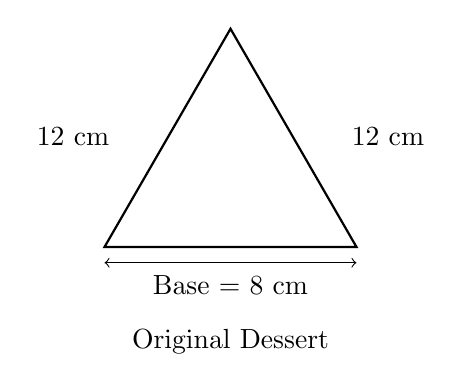
\begin{tikzpicture}[scale=0.4]
\draw[thick] (0,0) -- (8,0) -- (4,6.928) -- cycle;
\node at (4, -1.2) {Base = 8 cm};
\node at (9, 3.5) {12 cm};
\node at (-1, 3.5) {12 cm};
\draw[<->] (0,-0.5) -- (8,-0.5);
\node at (4, -3) {Original Dessert};
\end{tikzpicture}
\end{center}

    \ealpara{Oryginalny przepis używa:}{The original recipe uses:}
    \begin{itemize}
    \item \ealpara{120 g cukru (na \ealkeytr{pole})}{120g sugar (for the \ealkey{area})}
    \item \ealpara{80 g kakao w proszku (na dekorację \ealkeytr{obwodu})}{80g cocoa powder (for the \ealkey{perimeter} decoration)}
    \item \ealpara{3 jajka}{3 eggs}
    \end{itemize}
    \begin{enumerate}
    \item \ealpara{Jaki jest \ealkeytr{obwód} oryginalnego deseru?}{What is the \ealkey{perimeter} of the original dessert?}
    \item \ealpara{Jaki jest \ealkeytr{obwód} nowego, większego deseru?}{What is the \ealkey{perimeter} of the new, larger dessert?}
    \item \ealpara{Ile cukru potrzeba na większy deser?}{How much sugar is needed for the larger dessert?}
    \item \ealpara{Ile kakao w proszku potrzeba na większy deser?}{How much cocoa powder is needed for the larger dessert?}
    \item \ealpara{Ile jajek potrzeba na większy deser?}{How many eggs are needed for the larger dessert?}
    \end{enumerate}
\end{enumerate}

\newpage{}

\ealpara{Najlepsze zakupy -- przeszłość}{Best Buys Past}
\section*{Best Buys Past}

\begin{enumerate}[resume]
\item \ealpara{Pudełko płatków zbożowych 500 g kosztuje £4.50. Pudełko 750 g kosztuje £6.30. Który zakup jest lepszy?}{A 500g box of cereal costs £4.50. A 750g box costs £6.30. Which is the better buy?}

\item \ealpara{Sklep A sprzedaje 6 puszek napoju gazowanego za \$4.80. Sklep B sprzedaje ten sam napój z 15\% zniżką na pojedyncze puszki, które normalnie kosztują \$0.95 każda. Gdzie powinieneś kupić, jeśli potrzebujesz 6 puszek?}{Store A sells 6 cans of soda for \$4.80. Store B sells the same soda with a 15\% discount on single cans that normally cost \$0.95 each. Where should you buy if you need 6 cans?}

\item \ealpara{Butelka soku 2L kosztuje €3.20. Butelka 1.5L jest w promocji z 20\% zniżką od regularnej ceny €2.80. Który rozmiar oferuje lepszą wartość za litr?}{A 2L bottle of juice costs €3.20. The 1.5L bottle is on sale for 20\% off its regular price of €2.80. Which size offers better value per liter?}

\item \ealpara{\textbf{Electronic World} ma wyprzedaż:}{\textbf{Electronic World} is having a clearance sale:}
\ealpara{Słuchawki: pierwotnie £120, teraz 20\% zniżki}{Headphones: Original £120, now 20\% off}
\ealpara{Głośniki: pierwotnie £85, teraz 30\% zniżki}{Speakers: Original £85, now 30\% off}
\ealpara{Sklep prowadzi także promocję: kup 3 przedmioty, najtańszy gratis. Możesz sprzedać elektronikę lokalnemu sklepowi za 50\% ceny bez zniżki -- jaki jest najtańszy sposób, w jaki możesz kupić zarówno słuchawki, jak i głośniki?}{The store is also running a buy 3 items, get the cheapest free deal. You can sell electronics for 50\% of non-discounted price to a local shop - what is the cheapest way you can buy both the headphones and speakers?}

\item \ealpara{Sklep meblowy oferuje dwa plany płatności za sofę za £1200:}{A furniture store offers two payment plans for a £1200 sofa:}
\ealpara{Plan A: 25\% zadatku, potem 12 miesięcznych płatności po £80}{Plan A: 25\% down payment, then 12 monthly payments of £80}
\ealpara{Plan B: Bez zadatku, 18 miesięcznych płatności po £75}{Plan B: No down payment, 18 monthly payments of £75}
\ealpara{Biorąc pod uwagę całkowitą zapłaconą kwotę, który plan jest lepszy i o jaki \ealkeytr{procent} ceny pierwotnej?}{Considering the total amount paid, which plan is better and by what \ealkey{percentage} of the original price?}
\end{enumerate}

\vspace{2cm}

\ealpara{Najlepsze zakupy -- przyszłość}{Best Buys Future}
\section*{Best Buys Future}

\begin{enumerate}[resume]
\item \ealpara{Musisz ogrodzić prostokątny ogród. Sklep A sprzedaje ogrodzenie za \$12 za metr. Sklep B sprzedaje pocięte odcinki 2m za \$20 każdy. Co jest tańsze dla ogrodu 10m × 8m?}{You need to fence a rectangular garden. Store A sells fencing for \$12 per meter. Store B sells pre-cut 2m sections for \$20 each. Which is cheaper for a 10m × 8m garden?}

\item \ealpara{Chcesz położyć płytki na podłodze. Płytka typu A kosztuje £25 za metr kwadratowy. Płytka typu B kosztuje £18 za metr kwadratowy, ale wymaga 15\% więcej płytek z powodu stłuczek. Dla pokoju 4m × 5m, jaka jest najniższa cena położenia płytek w pokoju?}{You want to tile a floor. Tile Type A costs £25 per square meter. Tile Type B costs £18 per square meter but requires 15\% more tiles due to breakage. For a 4m × 5m room, what is the lowest price to tile the room?}

\item \ealpara{Farba kosztuje £35 za litr i pokrywa 12m² na litr. Marka X oferuje 20\% większe pokrycie na litr za £42 za litr. Do pomalowania dwóch ścian o \ealkeytr{wymiarach} 4m × 3m i 5m × 3m, która farba jest lepszą wartością? Kupując najtańszą, ile będzie kosztować farba?}{Paint costs £35 per liter and covers 12m² per liter. Brand X offers 20\% more coverage per liter for £42 per liter. For painting two walls of \ealkey{dimensions} 4m × 3m and 5m × 3m, which paint is better value? Buying the cheapest, how much will the paint cost?}

\newpage{}

\item \ealpara{Musisz kupić nasiona trawy na trawnik. Trawnik składa się z prostokąta (10m × 6m) z \ealkeytr{półkolistym} przedłużeniem (o \ealkeytr{promieniu} 3m) na jednym końcu. Nasiona A pokrywają 15m² na kg po \$4.80 za kg. Nasiona B pokrywają 25m² na kg po \$7.50 za kg. Które nasiona są bardziej ekonomiczne?}{You need to buy grass seed for a lawn. The lawn consists of a rectangle (10m × 6m) with a \ealkey{semicircular} extension (\ealkey{radius} 3m) at one end. Seed A covers 15m² per kg at \$4.80 per kg. Seed B covers 25m² per kg at \$7.50 per kg. Which seed is more economical?}

\begin{center}
\begin{tikzpicture}[scale=0.7]
\draw (0,0) rectangle (10,6);
\draw (10,0) arc (-90:90:3 and 3);
\draw (10,3) -- (10,0);
\node at (5,-0.5) {10m};
\node at (9.5 ,3) {6m};
\end{tikzpicture}
\end{center}

\item \ealpara{Basen ma następujący kształt: środkowy prostokąt 8m × 4m, z \ealkeytr{półkolistymi} końcami o \ealkeytr{promieniu} 2m. Musisz kupić pokrywę na basen. Materiał X kosztuje \$18 za m² i wytrzymuje 3 lata. Materiał Y kosztuje \$25 za m² i wytrzymuje 5 lat. Biorąc pod uwagę koszt roczny, który materiał jest bardziej ekonomiczny? Ile będzie kosztować rocznie utrzymanie basenu przykrytego za najniższą cenę?}{A swimming pool has the following shape: a central rectangle 8m × 4m, with \ealkey{semicircular} ends of \ealkey{radius} 2m. You need to buy a pool cover. Material X costs \$18 per m² and lasts 3 years. Material Y costs \$25 per m² and lasts 5 years. Considering cost per year, which material is more economical? How much will it cost per year to keep the pool covered for the least price?}

\begin{center}
\begin{tikzpicture}[scale=0.7]
\draw (0,0) -- (8,0);
\draw (0,4) -- (8,4);
\draw (0,0) arc (-90:90:2 and 2);
\draw (8,0) arc (-90:-270:2 and 2);
\node at (4,-0.5) {8m};
\node at (9,2) {4m};
\end{tikzpicture}
\end{center}

\end{enumerate}

\newpage{}


\ealpara{\ealkeytr{Skalowanie} -- przeszłość}{\ealkey{Scaling} Past}
\section*{\ealkey{Scaling} Past}

\begin{enumerate}[resume]

\item \ealpara{Rysunek jest \ealkeytr{skalowany} o 150\%. Jeśli pierwotna długość wynosiła 8 cm, jaka jest nowa długość?}{A drawing is \ealkey{scaled} up by 150\%. If the original length was 8 cm, what is the new length?}

\item \ealpara{\ealkeytr{Skalowanie} mapy wynosi 1:25,000. Jaki \ealkeytr{procent} rzeczywistej odległości reprezentuje 1 cm na mapie?}{A map \ealkey{scale} is 1:25,000. What \ealkey{percentage} of the actual distance does 1 cm on the map represent?}

\item \ealpara{Zdjęcie jest zmniejszone do 80\% swojej pierwotnej wielkości. Jeśli zmniejszona szerokość wynosi 12 cm, jaka była pierwotna szerokość?}{A photo is reduced to 80\% of its original size. If the reduced width is 12 cm, what was the original width?}

\item \ealpara{Sarah tworzy \ealkeytr{skalowany} rysunek swojej sypialni. Decyduje się użyć \ealkeytr{skalowania}, które reprezentuje 2\% rzeczywistego rozmiaru. Jaki \ealkeytr{stosunek} reprezentuje tutaj \ealkeytr{skalowanie}? Jeśli jej łóżko ma 2 metry długości w rzeczywistości, jaką długość powinna narysować na swoim \ealkeytr{skalowanym} rysunku? Podaj odpowiedź w centymetrach.}{Sarah is creating a \ealkey{scale} drawing of her bedroom. She decides to use a \ealkey{scale} which represents 2\% of actual size. What \ealkey{ratio} represents here \ealkey{scale}? If her bed measures 2 meters long in reality, what length should she draw it in her \ealkey{scale} drawing? Give your answer in centimetres.}

\item \ealpara{Firma produkuje \ealkeytr{skalowane} modele budynków. Model A jest wykonany w 2,5\% rzeczywistego rozmiaru, a Model B jest wykonany w 4\% rzeczywistego rozmiaru.}{A company is producing \ealkey{scale} models of buildings. Model A is made at 2.5\% of actual size, while Model B is made at 4\% of actual size.}
\begin{enumerate}
    \item \ealpara{Jeśli okno ma 1,2 metra szerokości w rzeczywistym budynku, jak szerokie jest w każdym modelu?}{If a window is 1.2 meters wide in the actual building, how wide is it in each model?}
    \item \ealpara{Jeśli wysokość Modelu A wynosi 45 cm, jaka jest wysokość rzeczywistego budynku?}{If Model A's height is 45 cm, what is the actual building's height?}
    \item \ealpara{O ile \ealkeytr{procent} większy jest Model B w porównaniu z Modelem A?}{What \ealkey{percentage} larger is Model B compared to Model A?}
\end{enumerate}

\end{enumerate}


\ealpara{\ealkeytr{Skalowanie} -- przyszłość}{\ealkey{Scaling} Future}
\section*{\ealkey{Scaling} Future}

\begin{enumerate}[left=0pt, start=11]

\item \ealpara{Kwadrat jest powiększony za pomocą \ealkeytr{współczynnika skali} 3. Jeśli pierwotny \ealkeytr{obwód} wynosił 12 cm, jaki jest nowy \ealkeytr{obwód}?}{A square is enlarged using \ealkey{scale factor} 3. If the original \ealkey{perimeter} was 12 cm, what is the new \ealkey{perimeter}?}

\item \ealpara{\ealkeytr{Skalowany} rysunek prostokątnego pola używa \ealkeytr{skalowania} 1:200. Jeśli rysunek pokazuje pole jako 6 cm × 4 cm, jakie jest rzeczywiste \ealkeytr{pole} tego pola?}{A \ealkey{scale} drawing of a rectangular field uses \ealkey{scale} 1:200. If the drawing shows the field as 6 cm × 4 cm, what is the actual \ealkey{area} of the field?}


\ealpara{Poniższy \ealkeytr{trójkąt równoboczny} przedstawia park. Jeśli każdy bok $s$ ma 2 cm na rysunku, znajdź:}{The \ealkey{equilateral triangle} below represents a park. If each side $s$ is 2 cm in the drawing, find:}
\begin{enumerate}
    \item \ealpara{Rzeczywisty \ealkeytr{obwód} parku}{The actual \ealkey{perimeter} of the park}
    \item \ealpara{Rzeczywiste \ealkeytr{pole} parku (\ealkeytr{pole} \ealkeytr{trójkąta równobocznego} = $\frac{\sqrt{3}}{4}s^2$)}{The actual \ealkey{area} of the park (\ealkey{area} of \ealkey{equilateral triangle} = $\frac{\sqrt{3}}{4}s^2$)}
\end{enumerate}

\begin{center}
\item 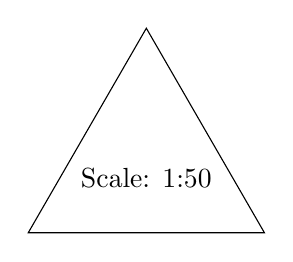
\begin{tikzpicture}[scale=0.5]
\draw (0,0) -- (6,0) -- (3,5.196) -- cycle;
\node at (3,1.4) {Scale: 1:50};
\end{tikzpicture}
\end{center}

\newpage{}

\item \ealpara{Plan przedstawia okrągłą fontannę o \ealkeytr{średnicy} 3 cm w \ealkeytr{skalowaniu} 1:30.}{A blueprint shows a circular fountain with \ealkey{diameter} 3 cm at \ealkey{scale} 1:30.}
\begin{enumerate}
    \item \ealpara{Jaka jest rzeczywista \ealkeytr{średnica} fontanny?}{What is the actual \ealkey{diameter} of the fountain?}
    \item \ealpara{Oblicz rzeczywiste \ealkeytr{pole} powierzchni fontanny.}{Calculate the actual \ealkey{area} of the fountain's surface.}
    \item \ealpara{Jeśli \ealkeytr{skalowanie} zmieniono na 1:45, jaka byłaby narysowana \ealkeytr{średnica}?}{If the \ealkey{scale} was changed to 1:45, what would be the drawn \ealkey{diameter}?}
\end{enumerate}

\item \ealpara{Architekt tworzy \ealkeytr{skalowane} rysunki dwóch \ealkeytr{podobnych} prostokątnych pokoi. Pokój A jest narysowany w \ealkeytr{skalowaniu} 1:100 i ma wymiary 5 cm × 4 cm na rysunku. Pokój B jest narysowany w \ealkeytr{skalowaniu} 1:80 i ma wymiary 6 cm × ? cm na rysunku.}{An architect creates \ealkey{scale} drawings of two \ealkey{similar} rectangular rooms. Room A is drawn at \ealkey{scale} 1:100 and measures 5 cm × 4 cm in the drawing. Room B is drawn at \ealkey{scale} 1:80 and measures 6 cm × ? cm in the drawing.}
\begin{enumerate}
    \item \ealpara{Oblicz rzeczywiste \ealkeytr{wymiary} i \ealkeytr{pole} każdego pokoju.}{Calculate the actual \ealkey{dimensions} and \ealkey{area} of each room.}
    \item \ealpara{Który pokój ma większe rzeczywiste \ealkeytr{pole} i o ile \ealkeytr{procent}?}{Which room has the larger actual \ealkey{area} and by what \ealkey{percentage}?}
    \item \ealpara{Jeśli oba rysunki zamieniono na \ealkeytr{skalowanie} 1:50, jakie byłyby ich nowe \ealkeytr{wymiary} na papierze?}{If both drawings were converted to \ealkey{scale} 1:50, what would be their new \ealkey{dimensions} on paper?}
\end{enumerate}

\end{enumerate}



\end{document}